\documentclass{article}
% \usepackage{tikz} 
\usepackage{pgfplots} 
\pgfplotsset{width=10cm,compat=1.9} 
 \usepgfplotslibrary{external} 
\usepackage[utf8]{inputenc}
\usepackage[linesnumbered,ruled]{algorithm2e}
\usepackage[margin=1.3in]{geometry}
 
 
\usepackage{hyperref}
\hypersetup{
    colorlinks=true,
    linkcolor=blue,
    filecolor=blue,      
    urlcolor=blue,
}
\urlstyle{same}
  
\usepackage{schemabloc}
\usetikzlibrary{circuits}

\usepackage[bottom]{footmisc}
\usepackage{pgf}
\usepackage{tikz}
\usetikzlibrary{arrows,automata}
\usepackage{verbatim}
 
\title{Capstone Report: Machine~Learning~for~Functional~Verification}
\author{Alberto Guasco}
\date{\today}
 
\begin{document}
 
\maketitle

 
\section{Definition}
% I. Definition
% 
% (approx. 1-2 pages)
In this report is described the project realized as conclusion of Machine Learning Nanodegree from Udacity. The project aims to use reinforcement learning for improving functional verification.

\subsection{Project Overview}
% Project Overview
% 
% In this section, look to provide a high-level overview of the project in layman’s terms. Questions to ask yourself when writing this section:
% 
%     Has an overview of the project been provided, such as the problem domain, project origin, and related datasets or input data?
%     Has enough background information been given so that an uninformed reader would understand the problem domain and following problem statement?
% 
The project consists in using reinforcement learning with actor-critic for improving the stress of a generic hardware. The project is under revision control using git at  \href{git@github.com:birio/capstone_project.git}{this remote} (git version 2.7.4) and has been developed using Python 3.5.2. This can be considered as the final work for showing what I learnt during the nanodegree. In my opinion the most important topic was reinforcement learning with actor-critic. This is a really recent method and it has been really interesting to see that all the references found were under intensive research work. Moreover, reinforcement learning with acotr-critic is needed for our goal beacuse of the high number of states. The environment used for developing our algorithm has been develpoed during the project (described in next section). The main goal is to test this cutting-edge technology with a generic and parametrizable environment. The project has been developed mainly with what has been done at Udacity, and using internet for various needs and suggestions (in the repository there's a file called \texttt{useful\_links.txt}).

\subsection{Problem Statement}
% Problem Statement
% 
% In this section, you will want to clearly define the problem that you are trying to solve, including the strategy (outline of tasks) you will use to achieve the desired solution. You should also thoroughly discuss what the intended solution will be for this problem. Questions to ask yourself when writing this section:
% 
%     Is the problem statement clearly defined? Will the reader understand what you are expecting to solve?
%     Have you thoroughly discussed how you will attempt to solve the problem?
%     Is an anticipated solution clearly defined? Will the reader understand what results you are looking for?
The problem we want to face is the functional verification of a random piece of hardware. Functional verification aims to ensure that a given RTL respects the specifications. The most difficult part of this work is to stress all possible states (and sequences of states) efficently, in order to save time and being sure that we are verifying mainly the most interesting states. What we normally want to ensure is that during verification RTL is continuosly stressed: this increase the probability to reach the bug condition. This is a very important topic because RTL is going to be more and more complex and the functional verification is the most time dispending phase of development. Reinforcement learning may help us in generating more intelligent stimuli. At each step (which corresponds to a clock cycle) we look at the state (which corresponds to the RTL register value) and then we decide the action (stimuli) to provide. What I would like to have is a generator which avoid invalid actions and is able to cover all possible states. 

\subsection{Metrics}
% Metrics
% 
% In this section, you will need to clearly define the metrics or calculations you will use to measure performance of a model or result in your project. These calculations and metrics should be justified based on the characteristics of the problem and problem domain. Questions to ask yourself when writing this section:
% 
%     Are the metrics you’ve chosen to measure the performance of your models clearly discussed and defined?
%     Have you provided reasonable justification for the metrics chosen based on the problem and solution?
In the domain of functional verification it's difficult to state that the design under testing (DUT) is fully verified. The level of verification is normally expressed using two indicators: how many tests have been run and the percentage of coverage reached. Coverage is a method in which a series of conditions (states values) is defined; the software used for testing collects how many times the DUT reached each of the conditions previously listed. The DUT model used for this project is done for returing also the coverage value at each step. In order to have a generic DUT, the coverage is defined as the list of all possible states and all possible transitions between states (when connected). This approach ensure us to see if the actions are stimulating all the possible functions of the DUT.  This metric is not used as reward during the reinforcement learning algorithm. The reward has been defined for ensuring an high coverage at the end of the test (high reward for high coverage) and for avoiding actions that doesn't change the state (negative reward for this actions, which are different for each state). The reward is used as feedback during reinforcement learning algorithm, while coverage is an index for understanding if at the end of a test (an episode) the DUT has been well explored: the goal is to have high exploration avoiding unallowed actions.

\section{Analysis}
% II. Analysis
% 
% (approx. 2-4 pages)

\subsection{Data Exploration}
% Data Exploration
% 
% In this section, you will be expected to analyze the data you are using for the problem. This data can either be in the form of a dataset (or datasets), input data (or input files), or even an environment. The type of data should be thoroughly described and, if possible, have basic statistics and information presented (such as discussion of input features or defining characteristics about the input or environment). Any abnormalities or interesting qualities about the data that may need to be addressed have been identified (such as features that need to be transformed or the possibility of outliers). Questions to ask yourself when writing this section:
% 
%     If a dataset is present for this problem, have you thoroughly discussed certain features about the dataset? Has a data sample been provided to the reader?
%     If a dataset is present for this problem, are statistics about the dataset calculated and reported? Have any relevant results from this calculation been discussed?
%     If a dataset is not present for this problem, has discussion been made about the input space or input data for your problem?
%     Are there any abnormalities or characteristics about the input space or dataset that need to be addressed? (categorical variables, missing values, outliers, etc.)
% 
Before starting the project, a python class for modeling the DUT has been developed. The class in file \texttt{Dut.py} aims to model a generic piece of hardware, assuming that any sequential logic can be modeled as a Moore's machine, so as a graph. Each node of the graph is a value of the Moore's state register. If it exists an input value for moving from a state to another one, the model has added the corresponding directed edge, having weight equal to the input value. With a little effort we are able to have a dataset for running our reinforcement learning algorithm. This allows us to have a DUT as big as needed, for sure without any functional bug, and can be used just for our neeeds:
\begin{itemize}
\item efficient: simulate a DUT and collect the coverage are particularly slow operations: with this approach we concentrate our computational effort on reinforcement learning only, without using any slow and apying software;
\item configurable: the Dut is generated with only two parameters, N\_STATES (total number of states) and N\_INPUTS (action bound is between 0 and N\_INPUTS - 1);
\item random: all connections are randomly generated;
\item flexible: it is use for generating a dataset and as environment capable of returning us the next state, rewards and coverage.
\end{itemize}
As previously described, a problem of functional verification is to always provide an input capable of stress the DUT. We have easly modeled this issue with unconnected states: in case of an action doesn't change the state.

The project is done using three configurations: 
\begin{center}
  \begin{tabular}{ | l | c | r | }
    \hline
      & N\_STATES & N\_INPUTS \\
    config\_1 &   32 &    8 \\
    config\_2 &  256 &   32 \\
    config\_3 & 1024 &  128 \\
    \hline
  \end{tabular}
\end{center}
Notice that the total number of coverage items is random.

Algorithm \ref{dut_algo} shows how the DUT is built. Notice that the class Dut is able also to return the next\_state given an action, and the coverage at each step. The main two dictionaries are DUT and COMB. For a given state \texttt{s}, \texttt{DUT[s]} returns the list of states connected to \texttt{s}. If \texttt{s\_0} and \texttt{s\_1} are connected, \texttt{COMB[s\_0, s\_1]} returns the input needed for moving from state \texttt{s\_0} to \texttt{s\_1}.

\begin{algorithm}[H]
 \SetKwInOut{Input}{Input}
 \SetKwInOut{Output}{Output}

 \Input{N\_STATES, N\_INPUTS}
 \Output{DUT, COMB}
 \For{all states s}{
  ensure that $s$ is reachable from almost one state \\
  define a random list $l$ of connected states \\
  DUT[$s$] = $l$
  \For{each next state $ns$ from list $l$}
  COMB[$s$, $ns$] = random(0, N\_INPUTS)
 }
 \caption{DUT model}
 \label{dut_algo}
\end{algorithm}

\subsection{Exploratory Visualization}
% Exploratory Visualization
% 
% In this section, you will need to provide some form of visualization that summarizes or extracts a relevant characteristic or feature about the data. The visualization should adequately support the data being used. Discuss why this visualization was chosen and how it is relevant. Questions to ask yourself when writing this section:
% 
%     Have you visualized a relevant characteristic or feature about the dataset or input data?
%     Is the visualization thoroughly analyzed and discussed?
%     If a plot is provided, are the axes, title, and datum clearly defined?
% 
We don't need a particular visualization of the Dut: the resulting graph may be particularly intricated (it is random) and in config\_2 and config\_3 it's really big. Moreover one of the initial hypothesis is that we don't need to know the DUT: we would like to build a reinforcement learning generator able to stress any DUT.

\subsection{Algorithms and Techniques}
% Algorithms and Techniques
% 
% In this section, you will need to discuss the algorithms and techniques you intend to use for solving the problem. You should justify the use of each one based on the characteristics of the problem and the problem domain. Questions to ask yourself when writing this section:
% 
%     Are the algorithms you will use, including any default variables/parameters in the project clearly defined?
%     Are the techniques to be used thoroughly discussed and justified?
%     Is it made clear how the input data or datasets will be handled by the algorithms and techniques chosen?
% 

The technique used for our goal is Reinforcement Learning. This approach has been chosen because of two reasons: it's the most interesting topic of the course, and it's the approach that most suits the issue, as we require an intelligent agent capable of generating a specific action for a given state.
\begin{algorithm}[H]
Algorithm parameters: step size $\alpha \in (0, 1]$ \\
Initialize $Q(s, a)$, for all $s \in \mathcal{S}^+, a \in \mathcal{A}(s)$, arbitrarily except that $Q(\mathrm{terminal}, \cdot) = 0$\;

\ForEach{episode}{
    Initialize S\;
    \ForEach{step of episode}{
        Choose $A$ from $S$ using policy derived from $Q$
        Take action $A$, observe $R$, $S'$\;
        $Q(S, A) \leftarrow Q(S, A) + \alpha [R + \gamma \max_a Q(S', a) - Q(S, A)]$\;
        $S \leftarrow S'$\;
    }
}
 \caption{Reinforcement Learning basic algorithm}
 \label{RL}
\end{algorithm}
Algorithm \ref{RL} shows a version of Reinforcement Learning: a key point is how to choose action $A$. The method chosen for our project is the \href{actor-critic}{https://arxiv.org/pdf/1509.02971v2.pdf}. With this approach we approximate both Q value function and the policy function with two neural networks. The training is done at each time step using a data saved in a dedicated buffer. The algorithm is particularly adapted for high dimensional environments. For the capstone project we have chosen this method because of it's really new and because DUT may have a very high number of states. An important point to underline is how reinforcement learning interacts with DUT:
\begin{itemize}
\item action: input value used for stimulating the DUT;
\item state: value of the DUT sequential logic at a given moment;
\item reward: indicator on the coverage;
\item step: unit of time (defined by the clock) in which DUT sample the input and compute the next state depending on the actual state.
\end{itemize}



\begin{figure}
\begin{center}
\tikzset{every picture/.style={line width=1pt}} %set default line width to 0.75pt        

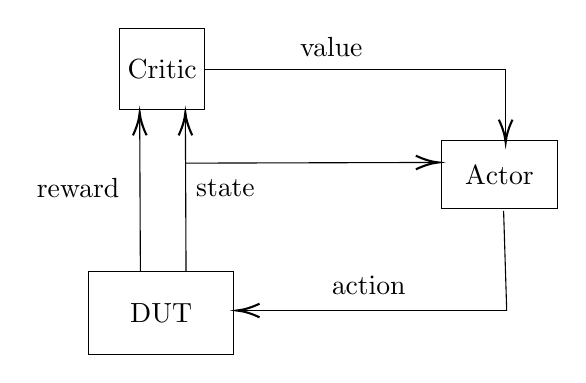
\begin{tikzpicture}[x=0.75pt,y=0.75pt,yscale=-1,xscale=1]
%uncomment if require: \path (0,300); %set diagram left start at 0, and has height of 300

%Straight Lines [id:da24848757761280937] 
\draw    (130,76) -- (275,76) ;


%Shape: Rectangle [id:dp41341892286088944] 
\draw   (244,110) -- (300,110) -- (300,143) -- (244,143) -- cycle ;
%Shape: Rectangle [id:dp8411018969332734] 
\draw   (89,56) -- (130,56) -- (130,95) -- (89,95) -- cycle ;
%Shape: Rectangle [id:dp474560766316674] 
\draw   (74,173) -- (144,173) -- (144,213) -- (74,213) -- cycle ;
%Straight Lines [id:da5893657999386903] 
\draw    (99,173) -- (98.68,98.67) ;
\draw [shift={(98.67,96.67)}, rotate = 449.75] [color={rgb, 255:red, 0; green, 0; blue, 0 }  ][line width=0.75]    (10.93,-3.29) .. controls (6.95,-1.4) and (3.31,-0.3) .. (0,0) .. controls (3.31,0.3) and (6.95,1.4) .. (10.93,3.29)   ;

%Straight Lines [id:da6125995597935853] 
\draw    (121,173) -- (120.68,98.67) ;
\draw [shift={(120.67,96.67)}, rotate = 449.75] [color={rgb, 255:red, 0; green, 0; blue, 0 }  ][line width=0.75]    (10.93,-3.29) .. controls (6.95,-1.4) and (3.31,-0.3) .. (0,0) .. controls (3.31,0.3) and (6.95,1.4) .. (10.93,3.29)   ;

%Straight Lines [id:da1672896739337899] 
\draw    (121,121) -- (240.67,120.67) ;
\draw [shift={(242.67,120.67)}, rotate = 539.8399999999999] [color={rgb, 255:red, 0; green, 0; blue, 0 }  ][line width=0.75]    (10.93,-3.29) .. controls (6.95,-1.4) and (3.31,-0.3) .. (0,0) .. controls (3.31,0.3) and (6.95,1.4) .. (10.93,3.29)   ;

%Straight Lines [id:da32551900771788567] 
\draw    (275,76) -- (275,109) ;
\draw [shift={(275,111)}, rotate = 270] [color={rgb, 255:red, 0; green, 0; blue, 0 }  ][line width=0.75]    (10.93,-3.29) .. controls (6.95,-1.4) and (3.31,-0.3) .. (0,0) .. controls (3.31,0.3) and (6.95,1.4) .. (10.93,3.29)   ;

%Straight Lines [id:da30346712534369324] 
\draw    (274,144) -- (275.5,192) ;


%Straight Lines [id:da17435101265626063] 
\draw    (275.5,192) -- (147.5,192) ;
\draw [shift={(145.5,192)}, rotate = 360] [color={rgb, 255:red, 0; green, 0; blue, 0 }  ][line width=0.75]    (10.93,-3.29) .. controls (6.95,-1.4) and (3.31,-0.3) .. (0,0) .. controls (3.31,0.3) and (6.95,1.4) .. (10.93,3.29)   ;


% Text Node
\draw (272,126.5) node  [align=left] {Actor};
% Text Node
\draw (109.5,75.5) node  [align=left] {Critic};
% Text Node
\draw (109,193) node  [align=left] {DUT};
% Text Node
\draw (140,133) node  [align=left] {state};
% Text Node
\draw (69,133) node  [align=left] {reward};
% Text Node
\draw (191,65) node  [align=left] {value};
% Text Node
\draw (209,179.83) node  [align=left] {action};


\end{tikzpicture}
\caption{Schematic of actor-critic approach}
\label{AC}
\end{center}
\end{figure}

\subsection{Benchmark}
% Benchmark
% 
% In this section, you will need to provide a clearly defined benchmark result or threshold for comparing across performances obtained by your solution. The reasoning behind the benchmark (in the case where it is not an established result) should be discussed. Questions to ask yourself when writing this section:
% 
%     Has some result or value been provided that acts as a benchmark for measuring performance?
%     Is it clear how this result or value was obtained (whether by data or by hypothesis)?
% 
Reinforcement learning results will be compared with the coverage obtained using a random generator. This kind of generator is commonly used as stimuli generator for functional verification: this in an heuristic method for searching the corner cases. This kind of generator have limited knowledge of the DUT and, most important, are not able to forecast the next state. It's then difficult to ensure that the DUT is sufficiently and uniformly explored. 
\begin{center}
  \begin{tabular}{ | l | r | }
    \hline
      & coverage \\
    config\_1 & 0.7377 \\
    config\_2 & 0.0667 \\
    config\_3 & 0.0033 \\
    \hline
  \end{tabular}
\end{center}
From the previous table we can see an important point: with bigger DUTs it's more difficult to have a good coverage, specially with completely random generation. 

\section{Methodology}
% III. Methodology
% 
% (approx. 3-5 pages)

\subsection{Data Preprocessing}
% Data Preprocessing
% 
% In this section, all of your preprocessing steps will need to be clearly documented, if any were necessary. From the previous section, any of the abnormalities or characteristics that you identified about the dataset will be addressed and corrected here. Questions to ask yourself when writing this section:
% 
%     If the algorithms chosen require preprocessing steps like feature selection or feature transformations, have they been properly documented?
%     Based on the Data Exploration section, if there were abnormalities or characteristics that needed to be addressed, have they been properly corrected?
%     If no preprocessing is needed, has it been made clear why?
% 
As previously explained, we don't have to do any data preprocessing. The DUT will be created at the beginning of the test and it uses a fixed seed for ensuring that the DUT is always the same at each run. We don't look at the DUT before the test and we don't have any need for searching or characterizing the dataset. The only property that we ensure at the creation of te DUT is that all states and all transitions are reachable.


\subsection{Implementation}
% Implementation
% 
% In this section, the process for which metrics, algorithms, and techniques that you implemented for the given data will need to be clearly documented. It should be abundantly clear how the implementation was carried out, and discussion should be made regarding any complications that occurred during this process. Questions to ask yourself when writing this section:
% 
%     Is it made clear how the algorithms and techniques were implemented with the given datasets or input data?
%     Were there any complications with the original metrics or techniques that required changing prior to acquiring a solution?
%     Was there any part of the coding process (e.g., writing complicated functions) that should be documented?
% 

As suggested during the review of Quadcopter project, the starting point of the project is from \href{this}{https://github.com/pemami4911/deep-rl.git} repository, where there the actor-critic algorithm has been implemented. Actor network has two hidden layers with 400 and 300 nodes each; critic network has two hidden layers for state input (400 and 300 nodes each), and one hidden layer for action input (300 nodes); the output (Q value approximation) is a combination of the two resulting layers. All activation functions of hidden layers are \texttt{relu}. The main functionalities are coded using \texttt{tflearn} API.

An important point consists in listing and managing main parameters used along the algorithm:
\begin{itemize}
\item neural network parameters:
\begin{itemize}
\item actor learning rate: learning rate of actor neural network;
\item critic learning rate: learning rate of actor neural network;
\item gamma: discount factor for critic updates;
\item tau: target weights update parameter;
\end{itemize}
\item replay buffer parameters:
\begin{itemize}
\item buffer-size;
\item minibatch-size;
\end{itemize}
\item general:
\begin{itemize}
\item max-episodes: number of episodes for learning;
\item max-episode-len: number of steps in each episode.
\end{itemize}
\end{itemize}

After having familiarized with the code, it was clear that we had to do big changes. First of all we have replaced the environment with the DUT: it has been easy becuase the DUT has been coded for being both a model and an environment. 

The first thing we had to think about, was the action. DDPG algorithm is structured in order to return a continuous value between two bounds. For our propose we need another format: for each discrete action value we need a value between 0 and 1, representing the probability that this action for a given state, may return a positive reward. At the end of learning the actor network, for a given state, will return a vector of N\_INPUTS elements, in which for each action there will be probability to have positive reward. This is needed because for a given state we may have multiple valid action to take, and we have to guarantee that our algorithm will take all valid actions for a given state.

A paper I used as reference has been \href{Deep Reinforcement Learning in Large Discrete Action Spaces}{https://arxiv.org/pdf/1512.07679.pdf}, were the policy had to return only one discrete action. The actor network return one real value, called \texttt{proto-action}, then we choose $k$ discrete values next to it, and with \texttt{KNN} algorithm they chose the discrete action with higher $Q$. This has been an important reference for me because I also need to transform the proto-action in something slightly different.

Another important topic is to manage the noise (which ensure us the randomness, so a good action exploration) with this specific action format. We can't use any discrete noise directly on the action to take, but we will add some noise on the probability of not-taken actions.

Similarly, state value has to be taken into account. Actor-critic consider the state as a continuous value, and the critic $Q$ value approximation is a function of both states and actions. Compared to our application, we have to really important differences:
\begin{itemize}
\item states are discretes: this will not require any correction to the algorithm;
\item $Q$ value functions of two close states can be completely independent between them: this becase the connection with other states are (pseudo) random.
\end{itemize}

This is not the only reason why it has been difficult to model the $Q$ value function. Differently from other reinforcement learning problem, in our project we don't have any fixed final state, or a clear optimal solution to follow, like a path in a maze. The optimal solution is the one which avoid unallowed actions, and that explore all possible states and connections, without doing too many times the same paths (quite similar to the traveling salesman problem). 

\subsection{Refinement}
% Refinement
% 
% In this section, you will need to discuss the process of improvement you made upon the algorithms and techniques you used in your implementation. For example, adjusting parameters for certain models to acquire improved solutions would fall under the refinement category. Your initial and final solutions should be reported, as well as any significant intermediate results as necessary. Questions to ask yourself when writing this section:
% 
%     Has an initial solution been found and clearly reported?
%     Is the process of improvement clearly documented, such as what techniques were used?
%     Are intermediate and final solutions clearly reported as the process is improved?
% 

Here there is the description of the main steps taken for having the final solution. The results refer to config\_1.

\subsubsection*{First step: make it works}
The first thing to do is to replace the environment with the DUT, and set the neural network input dimensions properly. Then we have to define how the reward is assigned: I assumed that the first approach to take is to be capable to distinguish between allowed and not-allowed actions for each state. Then I assigned $reward = 1$ in case the action returns a new $next\_state$, and $reward = -1$ in case we don't change $state$ after a step. Other kind of rewards have been tried, but this symmeric approach was the one that worked better. The second thing to do, as previously said, is to manage the action and its format. That's why we changed the last layer of the actor network: instead of returning a continuous value, we have put a $N\_INPUTS$  softmax output. Our expectation was to train the network for returning the probability for each possible action, and then choose the action as the following:
$$
action = np.random.choice(N\_INPUTS, p = softmax\_output)
$$
The results was surprising: with only 6 episodes the algorithm reaches the maximum possible reward, but, unfortunatly, with a really low coverage. What I discovered is that softmax is not good for setting multiple most-likely action, but it tends to promote only one element. That's why we reach high reward: it recognizes one action to take for each state, and then it always takes the same. Another important point is that we obtain the same results also adding some noise on softmax.
% initial solution
% softmax is not ok
% reward definition
% - SYMMETRIC

\subsubsection*{Second step: change activation function}
From previous step I assuemd that the approach taken was good, but we had to change (at least) the activation function. It implies that we can't use the network's output directly in the $choice$ function, but a normalization is needed, in order to have a vector that sum to one. The activation function has been chosen looking at the rewards at the end of each episode, and at the actions predicted for a given state, compared to the connections described in \texttt{COMB} and \texttt{DUT} dictionaries.
\begin{itemize}
\item relu: it predicted quite well one or more actions to take, but Q value exploded too fast;
\item relu6: it limits the Q value increase, but predictions saturated too fast without changing anymore;
\item tanh: worked quite well, but negative values added too many noise on predictions;
\item sigmoid: the one that worked better.
\end{itemize}
From udacity course we learned that the problem of sigmoid is that its derivative is too little when it tends to one or zero, resulting in a difficult learning. In order to avoid this problem, all activation function of actor hidden layers have been replaced using sigmoid.

The result was comparable to previous step, but quite randomly we had some degradation in terms of rewards. Looking at the $Q$ values for each episode, we saw that it didn't increase: it was decreasing or randomic. It suggested us that there was some randomness in the algorithm to manage.

\subsubsection*{Third step: heuristics for action selection and promotion}
We I had to improve is the action selection, which is described in algorithm \ref{action}. First of all we predict the action vector from the actor network; this is a vector of N\_INPUTS elements, where each element is between zero and one. The action to choose (for performing the step) is randomly chosen using as probability weights a normalized form of $probs$. Until now we can say that we have chosen the action returned from the actor network, but with some noise due to the random choise. The step will return a reward that has to be associated to the state and the action: which action? For being sure that the $probs$ vector corresponds to the action that returned a given reward, we have promoted the element $action$.


\begin{algorithm}[H]
probs = actor.predict(state) \\
action\_probs = [i/sum(probs) for i in probs] \\
action = np.random.choice(n\_inputs, p = action\_probs ) \\
probs[action] = 1 \\
 \caption{Action normalization and promotion}
 \label{action}
\end{algorithm}

Instead of using $choice$ function, we tried also $argmax$: as long as it doesn't add any noise, this approach produces less performing results. After this step the rewards and coverage were increasing reaching results comparable to random generation. We clearly needed to improve the performace.
% relu+sigmoid is not ok
% which action pass to train ?
% main algo with promotion
% actor network

\subsubsection*{Fourth step: states encoding}
As we discussed before, we have to put particular attention on states managing. At some point it was clear that we had to modify the networks in order to have each state independent with each other. We have discovered this needs looking at the most predicted actions per state: we saw that for a given state, an unallowed action had higher probability because of nearer states had that action as allowed. At the same time we don't want to build N\_STATES neural networks: it would be too costly and we would loose all actor-critic advantages.

The solution we have taken has been to add an $one\_hot\_encoding$ layer in both actor and critic network, right after the state input layer. With this approach for a given state, there will be just a portion of network that will be $turned on$. It has been an easy solution (maybe is not the ideal one for bigger DUT configurations) and it has been fast to see a little increase in learning.
%one_hot_encoding

\subsubsection*{Fourth step: adding bonus}
Bonus have been added keeping in mind two principles:
\begin{itemize}
\item avoid unallowed actions: negative rewards for unallowed actions;
\item exploration: returns some bonus when some coverage targets are reached.
\end{itemize}
\begin{algorithm}[H]
\If{next\_state == state}{
   reward = -1
}
\Else{
   reward = 1
}

\If{all actions have been covered for a given state}{
   reward = 5
}

\If{coverage  $\geq$ 0.5}{
   reward = reward + 5
}
\ElseIf{coverage $\geq$  0.6}{
   reward = reward + 10
}
\ElseIf{coverage  $\geq$ 0.7}{
   reward = reward + 100
}
\ElseIf{coverage $\geq$  0.75}{
   reward = reward + 500
}
\ElseIf{coverage $\geq$  0.8}{
   reward = reward + 2000
}
\ElseIf{coverage  $\geq$ 0.85}{
   reward = reward + 3000
}
\ElseIf{coverage  $\geq$ 0.9}{
   reward = reward + 5000
}
\ElseIf{coverage $\geq$  0.95}{
   reward = reward * reward
}

 \caption{Reward function}
 \label{rew}
\end{algorithm}
%some bonus
The final result is that we are able to increase both the rewards and the coverage. Please notice that in algorithm \ref{rew}, the expression $coverege \geq$ means that the the coverage $just$ overcome the threshold. The final result (commented in next section) was considered good, so we didn't search for any improvement.

\section{Results}
% IV. Results
% 
% (approx. 2-3 pages)

\subsection{Model Evaluation and Validation}
% Model Evaluation and Validation
% 
% In this section, the final model and any supporting qualities should be evaluated in detail. It should be clear how the final model was derived and why this model was chosen. In addition, some type of analysis should be used to validate the robustness of this model and its solution, such as manipulating the input data or environment to see how the model’s solution is affected (this is called sensitivity analysis). Questions to ask yourself when writing this section:
% 
%     Is the final model reasonable and aligning with solution expectations? Are the final parameters of the model appropriate?
%     Has the final model been tested with various inputs to evaluate whether the model generalizes well to unseen data?
%     Is the model robust enough for the problem? Do small perturbations (changes) in training data or the input space greatly affect the results?
%     Can results found from the model be trusted?
% 

We didn't perform any parameters evaluation, and we keep the ones as suggested from the papers. Moreover we didn't need any data manipulation: the algorithm is validated with three different DUT configurations.

Model evaluation has been done using a script that launch three times the algorithm, saving the stdout. The resulting logs have been parsed for extracting the results showed later in this report. As shown later, I'm confident (and happy) about the results mainly becasue of the high level learning trends: this translates in having both high rewards and coverage.

For a better characterization, we may run thousands of tests with random DUT (with the same configurations) and then see if coverage results and learning curves are similar.

\subsection{Justification}
% Justification
% 
% In this section, your model’s final solution and its results should be compared to the benchmark you established earlier in the project using some type of statistical analysis. You should also justify whether these results and the solution are significant enough to have solved the problem posed in the project. Questions to ask yourself when writing this section:
% 
%     Are the final results found stronger than the benchmark result reported earlier?
%     Have you thoroughly analyzed and discussed the final solution?
%     Is the final solution significant enough to have solved the problem?
% 

In the following table is resumed the most important outcome of our project. We can see that for config\_1 and config\_2, coverage is better when reinforcement learning is used. For config\_3 it's a little bit lower. We can state that this approach is good, it works as expected, but still needs some improvement for reaching higher coverage in smaller configurations, and for being more scalable for bigger ones.

\begin{center}
  \begin{tabular}{ | c | c | c | }
    \hline
      & Random & Reinforcement Learning \\
    config\_1 & 0.7377  & 0.8096 \\
    config\_2 & 0.0667  & 0.1004 \\
    config\_3 & 0.0033  & 0.0028 \\
    \hline
  \end{tabular}
\end{center}

The main justification is that we should scale the neural networks with the DUT size. Moreover my impression is that the layer $one\_hot\_encoding$ doesn't scale with big N\_STATES. Another important point is that we have to increase the number of step for bigger DUT: in the following table is resumed the number of coverage items per configuration, and is easy to see that 500 steps are not sufficient for config\_2 and config\_3 for reaching high coverage (as for random policy).

\begin{center}
  \begin{tabular}{ | c | c | }
    \hline
      & Coverage items \\
    config\_1 & 167 \\
    config\_2 & 1317 \\
    config\_3 & 53847 \\
    \hline
  \end{tabular}
\end{center}



% too little networks
% one hot doesnt scale
% insufficient number of steps for bigger duts

% script for looping
% visibly learning
% graphs
% 
% - random coverage means that we have something wrong
% - decreasing coverage mea means that we have something wrong
% - exploding Q  means that we have something wrong


\section{ Conclusion}
% V. Conclusion
% 
% (approx. 1-2 pages)

\subsection{Free-Form Visualization}
% Free-Form Visualization
% 
% In this section, you will need to provide some form of visualization that emphasizes an important quality about the project. It is much more free-form, but should reasonably support a significant result or characteristic about the problem that you want to discuss. Questions to ask yourself when writing this section:
% 
%     Have you visualized a relevant or important quality about the problem, dataset, input data, or results?
%     Is the visualization thoroughly analyzed and discussed?
%     If a plot is provided, are the axes, title, and datum clearly defined?
% 

The following graphs shows the rewards and coverage for each configuration.
\begin{itemize}
\item config\_1: the learning phase is really small; in the reward graph we can distinguish different areas due to the rewards bonus;
\item config\_2: the learning phase is really long, this may be due to the fact that 500 steps are too few for such DUT; coverage follows rewards expect for last 100 episodes (there isn't any reward bonus for this slow rewards);
\item config\_3: the neural networks are clearly too small for being able to model such a big DUT and both coverage and rewards are random.
\end{itemize}

\begin{center}
\begin{tikzpicture}
\begin{axis}[
title={config 1 - Rewards},
xlabel={Episodes},
ylabel={Rewards},
]
\addplot +[only marks, scatter] table
{ddpg_8_32_rewards.log};
\end{axis}
\end{tikzpicture}
\end{center}

\begin{center}
\begin{tikzpicture}
\begin{axis}[
title={config 1 - Covereage},
xlabel={Episodes},
ylabel={Coverage},]
\addplot +[only marks, scatter] table
{ddpg_8_32_coverage.log};
\end{axis}
\end{tikzpicture}
\end{center}

\begin{center}
\begin{tikzpicture}
\begin{axis}[
title={config 2 - Rewards},
xlabel={Episodes},
ylabel={Rewards},]
\addplot +[only marks, scatter] table
{ddpg_32_256_rewards.log};
\end{axis}
\end{tikzpicture}
\end{center}

\begin{center}
\begin{tikzpicture}
\begin{axis}[
title={config 2 - Covereage},
xlabel={Episodes},
ylabel={Coverage},]
\addplot +[only marks, scatter] table
{ddpg_32_256_coverage.log};
\end{axis}
\end{tikzpicture}
\end{center}

\begin{center}
\begin{tikzpicture}
\begin{axis}[
title={config 3 - Rewards},
xlabel={Episodes},
ylabel={Rewards},]
\addplot +[only marks, scatter] table
{ddpg_128_1024_rewards.log};
\end{axis}
\end{tikzpicture}
\end{center}

\begin{center}
\begin{tikzpicture}
\begin{axis}[
title={config 3 - Coverage},
xlabel={Episodes},
ylabel={Coverage},]
\addplot +[only marks, scatter] table
{ddpg_128_1024_coverage.log};
\end{axis}
\end{tikzpicture}
\end{center}


\subsection{Reflection}
% Reflection
% 
% In this section, you will summarize the entire end-to-end problem solution and discuss one or two particular aspects of the project you found interesting or difficult. You are expected to reflect on the project as a whole to show that you have a firm understanding of the entire process employed in your work. Questions to ask yourself when writing this section:
% 
%     Have you thoroughly summarized the entire process you used for this project?
%     Were there any interesting aspects of the project?
%     Were there any difficult aspects of the project?
%     Does the final model and solution fit your expectations for the problem, and should it be used in a general setting to solve these types of problems?
% 
The most interesting part of the project was try to imagine how each portion of the algorithm participate in learning, and then find a solution for improving each part. $Find a solution$ means searching everywhere: udacity, google scholar, blogs, friends and, most important, our brain. Moreover it has been fashinating to see how modern this topics are, and that this area still needs some stable and robusts bibliography.

More specific, I was really surprised on how the reward function determine the learning: I think that in future there will be a sort of function approximation just for improving this function in order to have a better learning.

\subsection{Improvement}
% Improvement
% 
% In this section, you will need to provide discussion as to how one aspect of the implementation you designed could be improved. As an example, consider ways your implementation can be made more general, and what would need to be modified. You do not need to make this improvement, but the potential solutions resulting from these changes are considered and compared/contrasted to your current solution. Questions to ask yourself when writing this section:
% 
%     Are there further improvements that could be made on the algorithms or techniques you used in this project?
%     Were there algorithms or techniques you researched that you did not know how to implement, but would consider using if you knew how?
%     If you used your final solution as the new benchmark, do you think an even better solution exists?
% 
% Before submitting, ask yourself. . .
% 
%     Does the project report you’ve written follow a well-organized structure similar to that of the project template?
%     Is each section (particularly Analysis and Methodology) written in a clear, concise and specific fashion? Are there any ambiguous terms or phrases that need clarification?
%     Would the intended audience of your project be able to understand your analysis, methods, and results?
%     Have you properly proof-read your project report to assure there are minimal grammatical and spelling mistakes?
%     Are all the resources used for this project correctly cited and referenced?
%     Is the code that implements your solution easily readable and properly commented?
%     Does the code execute without error and produce results similar to those reported?
% 
% 
% DO_MERGE = False

The problem solution appears to be good, but there space for improvement. It may be nice now to try with a verilog RTL, and see if it is capable, for example, to full stimulate a real not-random sequence of operations. Another study would imply the sampling of portion of the state (partially observable environment) as for real applications is too costly (the tests would be too long) to probes all the registers at each clock cycles.

Another intereting study would be to use a recurrent neural network, and then search for any solution to travel salesman problem, as done in \href{this paper}{https://arxiv.org/pdf/1611.09940.pdf}. 

\end{document}
